\section{Empirical application and results}\label{sec:results}
Evaluating the fitted policies on the target survey shows coarse trust-sign transfer, while agreement with human respondents remains unresolved. GPS supplies the anchors because its country scores are published aggregates of preference measures selected through prior experimental validation; they are not country-level collections of incentivized experimental choices. WVS Wave~7 serves as the target battery because it is a separate instrument, fielded on overlapping countries, whose items are candidate indicators for those same attributes. The item map is uneven on this panel, which makes the comparison informative: a policy trained on GPS signs can be tested for whether it retains those signs on WVS wording, and the same items can be tested for whether human country order agrees with GPS. Where the candidate map is weak, adapter--human disagreement can arise even when the construction successfully retains the anchor.

Three empirical comparisons structure the findings. First, on trust, a profile adapter with a neutral prompt transfers the coarse GPS sign. The country-prompt comparison is descriptive and appears below. Second, agreement with human country ranks on this panel remains unresolved, as does the candidate map's own association with the anchor across the same sixteen countries. Third, changing the evaluation prompt shifts both rank association and closeness to human response distributions, demonstrating sensitivity to configuration. The exhibits below provide the evidence for these three comparisons.

The diagnostic evaluation uses a purposively selected development panel of sixteen countries whose scores come from two saved jobs: Argentina, Brazil, China, Germany, Egypt, Great Britain, Greece, Indonesia, India, Japan, Mexico, Nigeria, the Netherlands, Russia, Turkey, and the United States. The first wave covers China, Japan, Great Britain, the United States, Mexico, Argentina, Germany, and Russia; the second covers India, Indonesia, Nigeria, Egypt, Turkey, the Netherlands, Brazil, and Greece. We assembled those waves to include both global sign polarities, the three duplicated sign profiles that share a labeling problem, mixed profiles, and geographic spread. The panel is not a probability sample of the forty-two-country GPS--WVS intersection. A later study that treats country selection as a sampling problem should train every country in that intersection or a predeclared random subset of it.

The primary comparison holds countries, item sets, recodes, and aggregation rules fixed across arms. It contains twenty-three single-choice items, including nine trust items. Egypt has no valid Q69--Q71 observations and Great Britain has no valid Q174 observations, so these items are removed everywhere. Q12--Q14 are multiple-response items and are excluded from the categorical softmax evaluation. Table~\ref{tab:map} lists the resulting map. Its proposed composites should not be read as validated measures of all six GPS traits. The original mapping preceded model scoring, whereas the strict common-support analysis and its sensitivity checks are retrospective.

\begin{table}[htbp]\centering\small
\caption{Candidate indicators on the strict common-support panel. Each row defines a candidate item set; latent-scale validity remains to be assessed. Patience items are interpreted separately.}\label{tab:map}
\begin{tabularx}{\linewidth}{@{}>{\raggedright\arraybackslash}p{30mm}>{\raggedright\arraybackslash}p{35mm}>{\raggedright\arraybackslash}X@{}}\toprule
Anchor & WVS items & Interpretation to be assessed\\\midrule
Trust & Q57--Q64, Q73 & Generalized, interpersonal, and institutional trust/confidence\\
Patience & Q43; Q50 & Less importance placed on work; financial satisfaction\\
Risk taking & Q106, Q107, Q109, Q178 & Economic values and fare avoidance\\
Positive reciprocity & Q81 & Confidence in charitable organizations\\
Negative reciprocity & Q176, Q177, Q179, Q195 & Moral clarity and justifiability judgments\\
Altruism & Q99, Q101, Q103 & Membership in environmental, charitable, and self-help groups\\\bottomrule
\end{tabularx}\end{table}

Generalized trust exhibits weak human--GPS agreement on the sixteen-country panel ($\rho = 0.15$ on Q57), underscoring that equivalence between each listed WVS item and its proposed GPS measure remains to be assessed. Q57 is the generalized-trust item related to the GPS validation comparison \cite{falk2018}. The wider trust composite pools substantively different items. The remaining mappings are exploratory bridges, especially where Wave~7 lacks direct counterparts to the preference benchmark.

\subsection{Recovery of the synthetic labels}
The country adapters instantiate thirteen distinct six-sign profiles across the sixteen countries (Table~\ref{tab:signprofiles}): Mexico shares its signs with Russia, India with Greece, and Indonesia with Egypt. Thus there are fewer distinct labeling problems than country labels. Each country adapter uses 526 training comparisons from a shared 658-pair bank, with 132 held-out comparisons. The fitting configuration uses $\beta=0.1$, LoRA rank 16 and scaling parameter 32, and one epoch. Appendix~\ref{app:training} records configuration and provenance limits.
\begin{table}[htbp]\centering\small
\caption{Thirteen distinct GPS sign profiles among the sixteen adapter countries. Coordinates are ordered trust, risk taking, patience, altruism, positive reciprocity, and negative reciprocity, matching Appendix~\ref{app:protocol}. The United States is non-negative on every coordinate; Mexico and Russia are negative on every coordinate. Identical sign vectors induce identical labels on the shared bank.}\label{tab:signprofiles}
\begin{tabular}{lcccccc}\toprule
Members & trust & risk & patience & altruism & pos.\ recip. & neg.\ recip. \\\midrule
EGY, IDN & $+$ & $-$ & $-$ & $+$ & $+$ & $+$ \\
GRC, IND & $-$ & $-$ & $-$ & $-$ & $-$ & $+$ \\
MEX, RUS & $-$ & $-$ & $-$ & $-$ & $-$ & $-$ \\
ARG & $-$ & $+$ & $-$ & $+$ & $+$ & $-$ \\
BRA & $-$ & $-$ & $-$ & $+$ & $+$ & $-$ \\
CHN & $+$ & $-$ & $+$ & $+$ & $+$ & $+$ \\
DEU & $-$ & $-$ & $+$ & $-$ & $-$ & $-$ \\
GBR & $+$ & $+$ & $+$ & $+$ & $-$ & $+$ \\
JPN & $-$ & $-$ & $+$ & $-$ & $-$ & $+$ \\
NGA & $-$ & $+$ & $-$ & $-$ & $-$ & $+$ \\
NLD & $+$ & $+$ & $+$ & $-$ & $-$ & $+$ \\
TUR & $+$ & $+$ & $-$ & $-$ & $-$ & $+$ \\
USA & $+$ & $+$ & $+$ & $+$ & $+$ & $+$ \\
\bottomrule
\end{tabular}\end{table}


Held-out evaluations confirm that the adapters learned the imposed synthetic contrasts. Pair-pooled across 2,112 held-out country--pair cells, the DPO margin-improvement rate is $0.942$ and pairwise synthetic-label accuracy is $0.819$. The former records a positive improvement in the chosen--rejected margin over the reference; the latter records a positive adapted-model margin itself. Country-level DPO margin-improvement rate ranges from $0.886$ to $0.992$. These results support recovery of imposed synthetic contrasts, but they do not measure prediction of independently observed choices. The inspected training notebooks record a shared seed-42 split of 526 and 132, but they do not record why Russia's holdout differs from that split. Fifteen countries share the seed-42 holdout; Russia's different 132-pair holdout shares 26 prompts with that set. This discrepancy limits the interpretation of pooled precision and country comparisons.

\subsection{Cross-survey associations}
Country-rank associations indicate marked differences between anchor retention and alignment with human respondents (Figure~\ref{fig:associations}). Table~\ref{tab:persona} supplies the country-named persona--GPS comparator. Country-bootstrap intervals use 2,000 common resamples and describe conditional within-panel stability given the fitted policies, GPS anchors, WVS point estimates, and selected items. They do not represent population sampling, respondent uncertainty, GPS measurement error, or training-seed variation, and are not multiplicity-adjusted. The intervals are wide because each association evaluates rank correlation across sixteen countries.

\begin{figure}[htbp]\centering
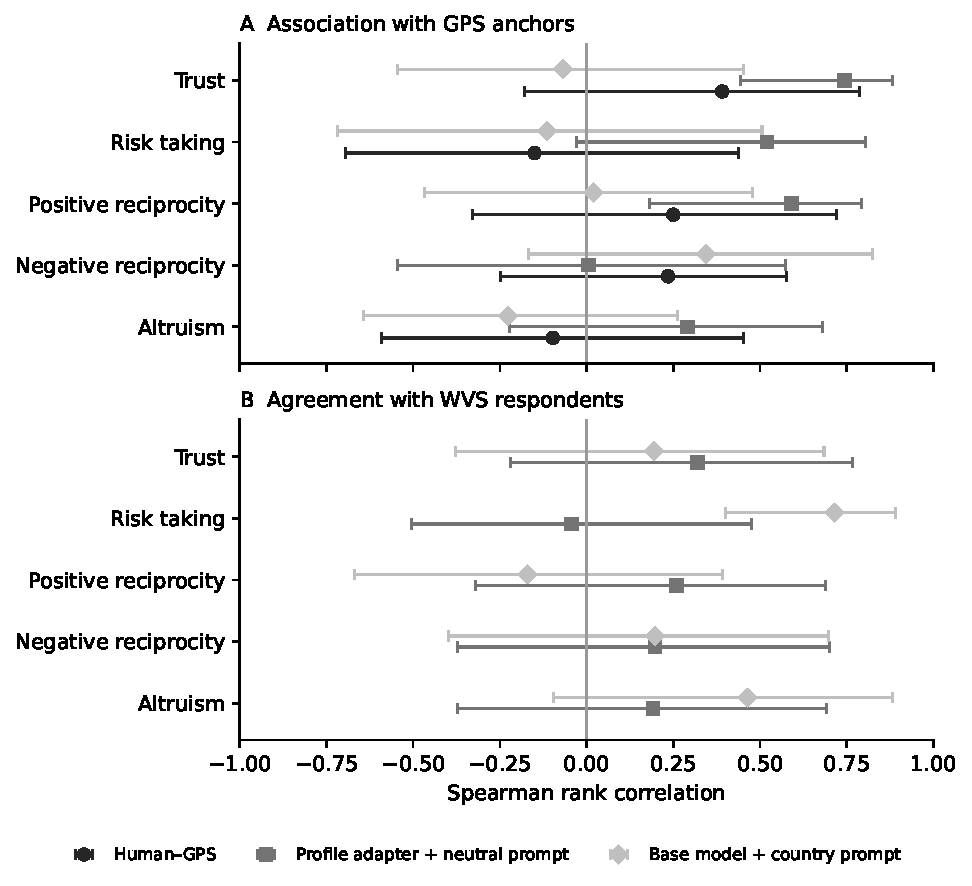
\includegraphics[width=\linewidth]{figures/associations.pdf}
\caption{Sixteen-country panel. Panel A is association with the GPS anchors. Panel B is agreement with WVS country responses. Markers are Spearman correlations; bars are 95\% country-bootstrap intervals from 2,000 resamples. The intervals are conditional within-panel stability summaries. They exclude training-seed variation, respondent resampling, and GPS measurement error. Patience is omitted because Q43 and Q50 are reported separately.}\label{fig:associations}
\end{figure}

On trust, profile adapters evaluated with a neutral prompt transfer the coarse GPS sign, with rank correlation $\rho = 0.74$ $[0.44, 0.88]$, compared with $-0.07$ for the country-prompted persona arm. The paired adapter-minus-persona difference is $0.81$ $[0.16, 1.31]$. The persona--GPS comparator is descriptive, with the caveat that identical checkpoints, tokenizers, code strings, and scoring procedures across historical runs were not established. Human--GPS association on the sixteen-country rectangle is $0.39$ $[-0.18, 0.79]$, whereas adapter--human association is $0.32$ $[-0.22, 0.77]$. The sixteen-country intervals leave human agreement unresolved, and they also leave the map's own criterion association unresolved. On the same nine-item recodes, the forty-two-country GPS--WVS intersection yields human--GPS association $0.35$ $[0.09, 0.56]$ (Table~\ref{tab:human42}). That larger human panel provides a criterion check on the map, but the adapters were not retrained on it. We draw no inference from similarity between a correlation and a product of other correlations, as that comparison does not identify an underlying mechanism.

A sign check on the trust composites establishes coarse trust-sign transfer across the purposively selected development panel. Seven countries have non-negative GPS trust anchors and nine have negative anchors. Adapter trust scores completely separate these two groups (rank-biserial correlation = 1.00) \footnote{A non-parametric measure that assesses the strength and direction of association between one binary (dichotomous) variable and one ordinal (ranked) variable}, with a mean between-group score difference of 0.43. We describe this result as coarse trust-sign transfer. The sixteen scores come from two saved jobs rather than a single evaluation run. The reported bootstrap intervals are conditional within-panel stability summaries; they do not reflect population sampling, respondent uncertainty, GPS measurement error, or training-seed variation.

In the tables, $\rho$ denotes the Spearman rank correlation across countries.
\begin{table}[htbp]\centering\small
\caption{Country-named persona--GPS association on the strict panel, with 95\% country-bootstrap intervals. This supplies the anchor comparator for Figure~\ref{fig:associations}.}\label{tab:persona}
\begin{tabular}{lcc}\toprule Anchor & $\rho$ & Interval\\\midrule
Trust & -0.07 & [-0.55, 0.45] \\
Risk taking & -0.11 & [-0.72, 0.51] \\
Positive reciprocity & 0.02 & [-0.47, 0.48] \\
Negative reciprocity & 0.34 & [-0.17, 0.82] \\
Altruism & -0.23 & [-0.64, 0.26] \\
\bottomrule
\end{tabular}\end{table}


Across the remaining preference dimensions, anchor retention and human agreement vary substantially by trait. For risk taking, adapter--GPS association on the two-wave scores is $0.52$ $[-0.03, 0.80]$, while adapter--human association is $-0.04$. Positive reciprocity yields an adapter--GPS association of $0.59$ and adapter--human association of $0.26$ on its single item (Q81). Altruism yields an adapter--GPS association of $0.29$ and adapter--human association of $0.19$. Negative reciprocity displays an adapter--GPS association of $0.01$ and adapter--human association of $0.20$. These divergences illustrate that anchor retention on one construct does not imply uniform transfer across all constructs. Mapping choices, anchor measurement, ecological differences, bank semantics, and scoring limitations can all contribute to divergence across dimensions.

\begin{table}[htbp]\centering\small
\caption{Patience candidate indicators, separately scored on sixteen countries. Entries are Spearman correlations; brackets give 95\% country-bootstrap intervals.}\label{tab:patience}
\begin{tabular}{lcc}\toprule Pairing & Q43 & Q50\\\midrule
Human--GPS & -0.56 [-0.86, -0.04] & 0.62 [0.11, 0.91] \\
Adapter--GPS & 0.01 [-0.47, 0.44] & 0.44 [-0.12, 0.79] \\
Adapter--human & 0.29 [-0.19, 0.73] & 0.25 [-0.32, 0.70] \\
Persona--GPS & -0.62 [-0.90, -0.10] & 0.62 [0.16, 0.87] \\
Persona--human & 0.59 [0.11, 0.82] & 0.70 [0.23, 0.91] \\
\bottomrule
\end{tabular}\end{table}

The two patience candidate indicators exhibit contrasting empirical patterns (Table~\ref{tab:patience}). On the two-wave scores, Q43 yields an adapter--GPS association of $0.01$ and adapter--human association of $0.29$, whereas Q50 yields an adapter--GPS association of $0.44$ and adapter--human association of $0.25$. The human--GPS correlations similarly diverge in sign: Q43 concerns reduced importance of work, whereas Q50 concerns financial satisfaction. We retain their original coding and report them separately rather than selecting a polarity after observing the correlations. Their two-item mean is an available computational summary, but it is not treated as a validated patience measure. The primary analysis therefore avoids aggregating them into a single composite.

\subsection{Distributional fit and prompt sensitivity}
Directional anchor retention and closeness to human response distributions do not favor the same configuration (Table~\ref{tab:twobytwo}). Evaluating the profile adapter with a neutral prompt achieves a trust--GPS association of $0.74$ and a mean total variation distance (TVD) of $0.487$ across 368 country--item cells. Adding a country prompt yields a trust--GPS association of $0.67$ and a mean TVD of $0.401$, though that trust cell was not recomputed from the two saved jobs. The base model with a country prompt achieves the lowest TVD ($0.369$), but exhibits no positive rank association with the anchor ($\rho = -0.07$).

\begin{table}[htbp]\centering\small
\caption{Configuration sensitivity on the strict panel. TVD averages 368 country--item cells. The Profile adapter + country prompt trust cell ($0.67$) was not recomputed from the two saved jobs. The base TVD uses banked runs. No base rank association with the anchor is interpreted, because run variation is confounded with the bank. Rank associations on this table use the same country bootstrap as Figure~\ref{fig:associations}, which excludes training-seed variation and GPS measurement error.}\label{tab:twobytwo}
\begin{tabular}{lcc}\toprule
Configuration & Trust--GPS $\rho$ & Mean TVD\\\midrule
Base model + neutral prompt & --- & 0.462\\
Base model + country prompt & $-0.07$ & 0.369\\
Profile adapter + neutral prompt & 0.74 & 0.487\\
Profile adapter + country prompt & 0.67 & 0.401\\\bottomrule
\end{tabular}\end{table}

Configuration sensitivity is trait-dependent, demonstrating that adding a country-specific prompt shifts both rank association and distributional fit. On risk taking, adding a country prompt alters the direction of association with the anchor and shifts alignment with human responses. These shifts describe configuration sensitivity rather than separating latent priors from anchor effects or establishing a general division between weights determining direction and prompts determining shape. The historical base runs also vary numerically despite identical saved prompts because they are not checkpoint-equivalent; they are therefore not treated as a single fixed base distribution. Identical checkpoints, tokenizers, code strings, and scoring procedures were not established across those runs, leaving comparisons with the base model descriptive.

The empirical evidence supports a fitted synthetic choice policy with trait-dependent external anchor association. Reliable prediction of human country ranks and practical pre-pilot benefits remain unestablished. We do not mix thirty-item total variation distance levels from earlier exploratory diagnostics with the strict-panel estimates, omitting that exhibit pending reconciliation of item eligibility and historical aggregation. A rank association alone cannot establish population dispersion.
